% !TEX root = ./Lemmen2024_modelingpractise.tex
%%
%% SPDX-FileCopyrightText: 2024 Helmholtz-Zentrum hereon GmbH
%% SPDX-FileCopyrightText: 2007-2020 Elsevier Ltd
%% SPDX-License-Identifier: LPPL-1.2
%% SPDX-FileContributor: Carsten Lemmen
%%%%
%% It may be distributed under the conditions of the LaTeX Project Public
%% License, either version 1.2 of this license or (at your option) any
%% later version.  The latest version of this license is in
%%    http://www.latex-project.org/lppl.txt
%% and version 1.2 or later is part of all distributions of LaTeX
%% version 1999/12/01 or later.
%%
%% The list of all files belonging to the 'Elsarticle Bundle' is
%% given in the file `manifest.txt'.
%%
%% Template article for Elsevier's document class `elsarticle'
%% with harvard style bibliographic references

\documentclass[preprint,11pt,5p]{elsarticle}

\usepackage{enumitem}
\providecommand{\tightlist}{%
  \setlength{\itemsep}{0pt}\setlength{\parskip}{4pt}}
\setlist[itemize]{leftmargin=*,labelsep=5.8mm}
\setlist[enumerate]{leftmargin=*,labelsep=4.9mm}

\usepackage[colorlinks=true]{hyperref}
\usepackage{calc}
\usepackage{longtable}
\usepackage{booktabs}
\usepackage{fancyhdr}
\usepackage{amsmath}
\usepackage{amssymb}

% Define page style with header on the first page
\fancypagestyle{firstpage}{
  \fancyhf{} % Clear header and footer
  \fancyhead[L]{\includegraphics[height=3cm]{./assets/elsevier-non-solus-new-with-wordmark.pdf}}
  \fancyhead[C]{submitted to Ecological Modelling}
  \fancyhead[R]{\includegraphics[height=3cm]{./assets/X03043800.jpg}}
  \renewcommand{\headrulewidth}{0pt} % Remove header rule
}

% definitions for citeproc citations
\NewDocumentCommand\citeproctext{}{}
\NewDocumentCommand\citeproc{mm}{%
\begingroup\def\citeproctext{#2}\cite{#1}\endgroup}
\makeatletter
% allow citations to break across lines
\let\@cite@ofmt\@firstofone
% avoid brackets around text for \cite:
\def\@biblabel#1{}
\def\@cite#1#2{{#1\if@tempswa , #2\fi}}
\makeatother
\newlength{\cslhangindent}
\setlength{\cslhangindent}{1.5em}
\newlength{\csllabelwidth}
\setlength{\csllabelwidth}{3em}
\newenvironment{CSLReferences}[2] % #1 hanging-indent, #2 entry-spacing
{\begin{list}{}{%
	\setlength{\itemindent}{0pt}
	\setlength{\leftmargin}{0pt}
	\setlength{\parsep}{0pt}
	% turn on hanging indent if param 1 is 1
	\ifodd #1
	\setlength{\leftmargin}{\cslhangindent}
	\setlength{\itemindent}{-1\cslhangindent}
	\fi
	% set entry spacing
	\setlength{\itemsep}{#2\baselineskip}}}
{\end{list}}
\newcommand{\CSLBlock}[1]{\hfill\break\parbox[t]{\linewidth}{\strut\ignorespaces#1\strut}}
\newcommand{\CSLLeftMargin}[1]{\parbox[t]{\csllabelwidth}{\strut#1\strut}}
\newcommand{\CSLRightInline}[1]{\parbox[t]{\linewidth - \csllabelwidth}{\strut#1\strut}}
\newcommand{\CSLIndent}[1]{\hspace{\cslhangindent}#1}

\journal{Ecological Modelling}

\begin{document}

\begin{frontmatter}
\thispagestyle{firstpage}

	%% use the tnoteref command within \title for footnotes;
	%% use the tnotetext command for theassociated footnote;
	%% use the fnref command within \author or \affiliation for footnotes;
	%% use the fntext command for theassociated footnote;
	%% use the corref command within \author for corresponding author footnotes;
	%% use the cortext command for theassociated footnote;
	%% use the ead command for the email address,
	%% and the form \ead[url] for the home page:
	%% \title{Title\tnoteref{label1}}
	%% \tnotetext[label1]{}
	%% \author{Name\corref{cor1}\fnref{label2}}
	%% \ead{email address}
	%% \ead[url]{home page}
	%% \fntext[label2]{}
	%% \cortext[cor1]{}
	%% \affiliation{organization={},
	%%            addressline={},
	%%            city={},
	%%            postcode={},
	%%            state={},
	%%            country={}}
	%% \fntext[label3]{}

\title{Good Modelling Software Practices}

%% use optional labels to link authors explicitly to addresses:
%% \author[label1,label2]{}
%% \affiliation[label1]{organization={},
%%             addressline={},
%%             city={},
%%             postcode={},
%%             state={},
%%             country={}}
%%
%% \affiliation[label2]{organization={},
%%             addressline={},
%%             city={},
%%             postcode={},
%%             state={},
%%             country={}}

\author%
[1]%
{%
%\href{https://orcid.org/}{
\includegraphics[width=1em]{./assets/logo-orcid-eps-converted-to}}\,
Carsten Lemmen\corref{carsten.lemmen@hereon.de}}
\author%
[2]%
{%
%\href{https://orcid.org/}{
\includegraphics[width=1em]{./assets/logo-orcid-eps-converted-to}}\,
Philipp Sebastian Sommer}

\affiliation[1]{Institute of Coastal Systems - Analysis and Modeling,
Helmholtz-Zentrum Hereon, Max-Planck-Str. 1, 21502 Geesthacht, Germany}
\affiliation[2]{Institute of Carbon Cycles, Helmholtz Coastal Data
Center, Helmholtz-Zentrum Hereon, Max-Planck-Str. 1, 21502 Geesthacht,
Germany}

\begin{abstract}
In socio-environmental sciences, models are frequently used as tools to
represent, understand, project and predict the behaviour of these
complex systems. Along the modelling chain, Good Modelling Practices
have been evolving that ensure -- amongst others -- that models are
transparent and replicable. Whenever such models are represented in
software, good modelling meets Good software Practices, such as a
tractable development workflow, good code, collaborative development and
governance, continuous integration and deployment, and Good Scientific
Practices, such as attribution of copyrights and acknowledgement of
intellectual property, publication of a software paper and archiving.
Too often in existing socio-environmental model software, these
practices have been regarded as an add-on to be considered at a later
stage only; in fact, many modellers have shied away from publishing
their model as open source out of fear that having to add good practices
is too demanding. We here argue for making a habit of following a list
of simple and not so simple practices early on in the implementation of
the model life cycle. We contextualise cherry-picked and hands-on
practices for supporting Good Modelling Practices, and we demonstrate
their application in the example context of the Viable North Sea
fisheries socio-ecological systems model.
\end{abstract}

%%Graphical abstract

%%Research highlights

%--
%% Keywords
%%% keywords here, in the form: keyword \sep keyword
%%% PACS codes here, in the form: \PACS code \sep code
%%% MSC codes here, in the form: \MSC code \sep code
%%% or \MSC[2008] code \sep code (2000 is the default)
\begin{keyword}
Good Modeling Practice\sep
Good Software Practice\sep
Good Scientific Practice\sep

\end{keyword}

\date{\today}
\end{frontmatter}

\section{Introduction}\label{introduction}

In socio-environmental sciences, models are frequently used as tools to
represent, understand, project and predict the behaviour of these
complex systems. The degree of a model's formalization ranges from
conceptual to mathematical equations to implementation in software,
and--by definition--all of these models are purpose-driven
simplifications of the system they represent (Stachowiak 1973;
Romanowska 2015). We here concentrate on computational models, i.e.~on
socio-environmental models implemented in software, and there are many
of those out there: Currently the CoMSES Network lists 1117 models
(Network for Computational Modeling in the Social and Ecological
Sciences 2024a); A. B. G. Janssen et al. (2015) asked 42 modelers about
their inventory of aquatic ecosystem models and came up with a list of
278 different models, more than a decade after Benz, Hoch, and Legović
(2001) counted some 1360 ecological model softwares.

So computational models are plenty and omnipresent in our field. But
despite their undoubted value, they have been criticised as
``unscientific'', as they often escape a strict requirement of
falsifiability: the code may be verifiable only within certain accuracy
ranges but not universally; the model may be validated only in
site-specific application but not universally (Refsgaard and Henriksen
2004). So all we can do is to provide at best verified and validated
models, and Good Modelling Practices (GMP) aim at ensuring this.
Examples of such practices often named are: a clear purpose, a thorough
domain understanding, going from simple to complex, ensuring
reproducibility, exploring sensitivities and validation with good
quality data (e.g., Crout et al. 2008). The first reference to this may
have been by Smagorinsky (1982), who claimed that ``under any
cirumstance, good modeling practice demands an awareness of the
sensitivity {[}{]} to parametrization'' (p.16). From here on, GMP were
elaborated and became widespread in the field of hydrology, with the
first handbook on the topic by Van Waveren (1999); it has since been
applied to all areas of socio-environmental sciences and has been
adopted in community standards such as the Overview, Design, Detail
(ODD) documentation protocol and its derivatives (Grimm et al. 2006,
2010, 2020).

Good Modeling Practices appear as five phases in the model life cycle
(Table 1 of Jakeman et al. 2024): (1) Problem scoping and (2)
conceptualization, (3) Model formulation and evaluation, (4)
application, and (5) perpetuation, and the reiteration of these phases.
Good Modelling Software Practices (GMSP) are prominent in phases 3--5,
and are thus subsumed under GMP. But where GMP is concerned with the
reliability and validity of a model --- possibly foremost its purpose,
scope and assumptions (Wang et al. 2023) --- GMSP is concerned with the
quality and reliability of a model's software implementation and beyond:
a good quality model software is not restricted to good computer code,
but can also aid to support iterations through the model life cycle and
help to follow Good Scientific Practice (Commission on Professional Self
Regulation in Science 2013).

Other scientific and technical fields where software plays a major role
developed the concept of Good Software Practice, which can be traced
back to the origins of the Unix systems, which has at its core not a
monolithic but highly granular structure of many little programs that
``do one thing only, and do it well'' (Ritchie and Thompson 1974). These
little tools should allow to develop new software in a better way,
argued B. W. Kernighan and Plauger (1976), for example by following the
DRY principle: ``Do not repeat yourself'', and to KISS --- ``keep it
simple, stupid!'' (Stroop 1960; Raymond 2003). Cotemporaneously the Free
Software movement emerged to emancipate software from the ownership of
companies and consider it a public good, which can be (1) run for any
purpose, (2) studied and modified, (3) distributed, and (4) modified and
distributed (Stallman 1983, 1996), and with it the practices to ensure
these freedoms in Open Source software. Educating about good practices
became central in projects such as the Software Carpentry (Wilson 2016),
highlighting the utility of live coding, pair programming and ``open
everything''.

``Better software, better research'' is a slogan by the Software
Sustainability Institute (SSI), promoting planning, development,
reliability, performance and collaboration in research software, and
advocationg for the recognition of the work of the people that develop
such software but are often not acknowledged in publications as the
major form of scientific output -- the Research Software Engineers (RSE)
(Katz et al. 2019; Hettrick et al. 2022). International agreements
require that research data must be Findable, Accessiple, Interoperable,
and Reusable (Wilkinson et al. 2016). Consequently, also software should
be FAIR: (F) easy to find; (A) retrievable via standardised protols; (I)
interoperates with other software by data exchange or an application
programming interfaces (API), and (R) can be understood, modified, built
upon, or incorporated into other software (Barker et al. 2022). Research
organizations like Network for Computational Modeling in the Social and
Ecological Sciences (2024b) educate about FAIR research software,
including rich metadata, code management, archiving, documentation, and
licensing. And it has been argued that some good practices around data
managment, software organization, collaboration, project organization,
change tracking, and manuscripts may be good enough (Wilson et al.
2017). Together, good practices in modelling, software development, and
research form a triangle with GMSP at its center
(\hyperref[fig:triangle]{Figure 1}).

\phantomsection\label{fig:triangle}
\begin{figure}
\centering
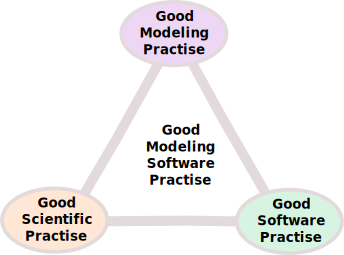
\includegraphics{Figure_1.pdf}
\caption{The triangle formed by good practices in modelling, software
and research \label{fig:triangle}}
\end{figure}

Despite these published best practice guidelines, much of the model
source code corpus, roughly 80\% (Barton et al. 2022) is not published
at all along with the scientific publication, and for a trivial reason:
Barnes (2010)'s survey stated that ``the code is a little raw'' was
named as the main reason for not publishing the model. Here we aim to
address this fear and help build confidence that the model code is good
enough in line with Wilson (2016) and Barnes (2010); beyond those, we
break them down to concrete recipes on how to implement those good
practices during the modelling software creation process. We start off
by motivating each of the good practices and contextualizing them
towards the goal of publishing a model software or a scientific result
arising from model software. We describe the tools that can be used in a
non-exhaustive way covering the entire range of good practices. You may
deviate from the tools we selected, or disagree with them, and you may
add others or leave some out that we suggested.

\subsection{Structure}\label{structure}

All models start with a purpose. That has since long bin the number one
Good Modelling Practice advice put forward. It doesn't hurt to know
about your domain, either, and most often a scientific software is
developed by a domain expert (Wilson 2016). Speak to other experts,
develop a conceptual model, only then start formalizing your model in
math and in software (Wang et al. 2023; Romanowska 2015; Grimm et al.
2006) to arrive at at your computational model -- a purpose-driven and
simplified representation of your system in software.

Socio-environmental modelling software can be created by a \emph{single
person}; in fact, it often is in student or postdoc projects or
individual programming sprints (Hettrick et al. 2022). Unfortunately
from a software developing perspective, the necessity of having to be a
domain expert at the same time means that 90\% of scientists are
self-taught developers without formal training in software engineering
(Wilson 2016). That one person will have to read her own code and to
apply it for simulations, she will have to align the software
development with her research, will have to understand what she did in
the past, she will have to retrace the steps that led her to the current
state. All of this necessitates to some degree that the work is stored
redundantly in backups, and that changes are documented. She would like
to ensure that code changes do not break previous work, and does that by
testing the model after every update (Rosero, Gómez, and Rodríguez
2016).

If the model is to be used to produce scientific results subject to
\emph{peer review}, the single person will have to ensure replicability
of results. She will have to subject it to an editor or a reviewer, thus
make it readable, and document it. And sometimes, she might be asked to
support the reviewers in executing the model somewhere outside her own
computer infrastructure. When feedback comes, there should be a platform
to file the individual concerns and address them.

If at least one \emph{other person} is using the model, the permission
issue --- also known as the license -- becomes pertinent. This other
user needs a way to communicate with the developer, for feature requests
or for reporting bugs. If that person intents to improve on your work,
the permissions become more important, needing contributor agreements
and codes of conduct. How are decisions made about the now joint
modelling software -- some form of governance model needs to be
established. With the growth of a community, even a community management
system might be required, with granular access, distributed roles, and
fine-grained permissions.

Regardless of the size of the collaboration, structured reviews,
pre-commit hooks, and common coding standards can be used to maintain
high code quality. Software needs to be sustainable as you aim for
establishing a larger user base, use it in other scientific software,
but most importantly, use the model to support scientific conclusions:
Good Scientific Practice demands that primary data are available for a
minimum of 10 years after when a scientific publications relies on them,
and so should models (Commission on Professional Self Regulation in
Science 2013). This is often a difficult requirement when models are
developed in externally funded projects, when hardware and software
environment change, or where mobility requirements demand for
relocations of staff and frequent change of jobs. Mobility is a good
argument in such circumstances for releasing your model as Free and Open
Source Software (FOSS) so that the developer herself can take it along.

\subsubsection{Single authors}\label{single-authors}

Authors of scientific models eventually become authors or co-authors of
scientific publications arising from or with the help of a model. As
scientific authors, they are bound by ethical considerations such as the
Guidelines for Safeguarding Good Scientific Practice, among them the
unambiguous declaration of intellectual property to the work and
ensuring availability of the model for a prolonged period of time
(Commission on Professional Self Regulation in Science 2013). The
declaration of intellectual property carries with it the proper
acknowledgement of software the model is built on, and respecting the
permissions pertaining to the sources used. The archiving requirement
carries with it the obligation to ensure that technical failures or
changes in the circumstances of the model author do not lead to the loss
of the model: decentralized backups or public repositories help.

For many scientific model authors, getting stuff done may be more
important than documenting it thoroughly, usefulness is more valued than
red tape, spontaneous ideas are implemented preferably over those layed
down in a management plan; individual agency supersedes organizational
processes. In this way, scientific model software development reflects
the ideas formulated in agile development: ``Individuals and
interactions over processes and tools. Working software over
comprehensive documentation. Customer collaboration over contract
negotiation. Responding to change over following a plan'' (Beck et al.
2001). And while the items on the left are valued more, the items on the
right are still important.

There are many tools available to structure and ameliorate the work for
the less preferred actions. Some that help with clarifying legal
constraints and documentation, and others that help with structuring the
development process, among them source code management services. One
criterion to assess whether software is sustainable is the truck factor,
asking: ``How many people can get hit by a truck, before the project
becomes unmaintainable?''; the OpenSSF gold standard requires that is
truck factor is \(>= 3\) (Open Source Security Foundation 2024).

\subsubsection{Reviewers}\label{reviewers}

To be published in a scientific journal, reviewers need to be able to
access and understand the model. Various documentation principles can
help to ensure this accessibility, including automatically generated
application programming interface (API) references, in-code
documentation and the generation of metadata through packaging. Advice
on how to write the code is old and simple: ``Write code that minimizes
the time it would take someone else to understand it---even if that
someone else is you.'' (Flesch 1950).

But even before a reviewer invests her time in evaluating a model
software, much can be done in advance by the author herself. In fact,
where a reviewer might concentrate on model validation, the author could
ensure model verification (Sargent 1994). Verification answers the
questions: Does the code do what the author intends it to do? To ensure
this, it has become good software practice to employ unit testing and
try to reach a good coverage of the test framework over your entire code
base (Ellims, Bridges, and Ince 2006), and to integrate automated
verification with the source code management service as Continuous
Integration (CI, Shahin, Ali Babar, and Zhu 2017).

How does an author deal with the feedback she receives during a friendly
or journal-led review? Often, this comes as an itemized list of points
to address; as such it is in an ideal form to be converted to
\emph{tickets} or \emph{issues} in the SCM service, or a dedicated issue
tracker system linked to the model software. Improvements to the model
code can then be tied to the issue tracker, transparently documenting
the resolution of those issues, and helping to formulate the rebuttal to
reviewer critique.

\subsubsection{Collaborators}\label{collaborators}

While most reviewers may only need passive (read) access to the
software, it is often desirable to collaboratively develop the software,
i.e.~involve another person or persons in improving the software. With
this collaboration come legal and governance decisions, as well as
technical requirements. The legal once concerns copyrights of the
different contributors, and often of the employers (research
organizations): Many academic institutions do not have yet clear
guidelines on the legal aspects of how to contribute to collaborative
software or how to accept contributions by other institutions. These can
be established in contributor agreements.

For collaborative development with a smaller group, a governance system
known as the benevolent dictator is frequently encountered. A benevolent
dictator in software development refers to a leadership style where one
individual, often the project's creator or lead developer, has
significant control over decision-making processes within the project.
Despite holding considerable authority, this individual typically
exercises their power with the best interests of the project and its
community in mind, hence the term ``benevolent.'' This leadership model
aims to maintain direction and cohesion within the project while still
allowing for contributions and feedback from other team members or
contributors (Schneider 2022). In scientific projects, the governance
and licensing terms for a collaboration can be formulated as part of a
Memorandum of Understanding or consortium contract.

\section{Tools for Good Modelling Software
Practice}\label{tools-for-good-modelling-software-practice}

The tools described here can roughly be categorized as version control,
source code management system, licensing, documentation, packaging, good
code, archiving and maintenance, and publication.

\subsection{Version control software}\label{version-control-software}

A transparent and reproducible distributed source code management (SCM,
a modern term for version control system, VCS) is the basis for good
software and has been termed ``possibly the biggest advance in software
development technology'' (Spolsky 2010). The dominant SCM software is
Git\footnote{https://git-scm.com open source distributed VCS Git. Note:
  all URLs in this manuscript have been last visited and checked on May
  31, 2024.}, originally invented by Linus Torvalds, the creator of
Linux. As source code is text, the SCM tracks changes in lines or parts
of lines of text. It can be very well used to manage other kinds of
changing texts, such as the text of this manuscript. In fact, this
manuscript was started with \texttt{git} \texttt{init;} \texttt{git}
\texttt{add\ manuscript.md;} \texttt{git} \texttt{commit} \texttt{-m}
\texttt{"Created\ manuscript"}, and has been evolving with repeated
recording of small changes à la \texttt{git} \texttt{add} \texttt{-u;}
\texttt{git} \texttt{commit} \texttt{-m} \texttt{"Added\ section"}, with
descriptive texts in quotation marks, the so-called commit messages.

With graphical interfaces to Git, such as Sourcetree\footnote{https://www.sourcetreeapp.com
  free Git client}, or various integrations in text editors, such as
Visual Studio Code\footnote{https://code.visualstudio.com editor with
  built-in Git}, it is now easy to follow the step-wise development of
code (or text documents), go back to points in time or critical
development stages, to open experimental deviations from main
development (\texttt{git} \texttt{branch}) and combine diverging
developments (\texttt{git} \texttt{merge}). Did you mess up? Simply
retrace your step back \texttt{git} \texttt{revert}; it helps you even
to find in the recorded history those developments where things might
have unnoticingly gone wrong with \texttt{git} \texttt{bisect}.

Git and others are most powerful as distributed VCS, in combination with
other locations on your own computer, an intranet or the internet, for
saving your work in different places, the \emph{repositories}, while
keeping all those versions synchronized. The interaction of two
repositories is managed by the unidirectional synchronizations
\texttt{git} \texttt{pull} and \texttt{git} \texttt{push}. These
commands can be used to synchronize the managed code also across
different SCM services, effectively allowing redundant and distributed
backups minimizing the risk of losing the software from technical or
human errors or the risk of vendor lock-in (Nyman and Lindman 2013).

\subsection{Source code management
service}\label{source-code-management-service}

The most prominent online SCM service is GitHub\footnote{https://github.com
  Public GitHub}, but many academic institutions also offer on-premise
or cross-institutional dedicated SCM services, such as the community
GitLab of the German Helmholtz Association\footnote{https://codebase.helmholtz.cloud.de
  Community Gitlab of the German Helmholtz Association} for their
students and researchers. A good reason to choose GitHub is the higher
amount of potential contributors on this platform; on-premise GitLabs
may be preferred by academic institution, because the code is then
hosted in the research center or by a dedicated subcontracted partner
and may offer better data protection, or because of dedicated CI
resources. This online platform serves as the entrypoint for
collaborators to contribute, provides a ticketing system and release
management, and offers functionalities for continuous integration and
continuous deployment of the software.

\subsubsection{Ticketing system}\label{ticketing-system}

Often things don't work right away, or an error is detected in the
software. For this, SCM services offer ticketing (also called bug
tracker or issue tracking) systems, where one records the occurrence of
an error, a \emph{bug report}, or a wish for future development, a
\emph{feature request}. This works well for a single person, but even
better when collaborators and reviewers of the software record their
observations on faulty or missing issues with the software on this
ticketing system. Beyond the ticketing system, the SCM service may also
offer communication facilities like discussion forums, wikis, mailing
list or service desks, which often provide cross-referencing
functionality to Git commits and issues.

\subsubsection{Continuous integration and
deployment}\label{continuous-integration-and-deployment}

CI is a development practice where developers integrate code into a
shared repository frequently, ideally several times a day, but at least
on every \texttt{git} \texttt{push} to a repository. Each integration is
then verified by an automated build and automated tests to detect errors
as quickly as possible; the frequent and automated check reduce the risk
of accumulating errors. SCM services like GitLab or GitHub provide such
automated integrations, called ``Actions'' on GitHub, but there are many
CI tools available outside the comprehensive SCM services, such as
Circle CI\footnote{Circle CI https://circleci.com}. CD is often
triggered after the CI ends with success. In this automation, the
products of a modelling software can be provisioned, such as a complete
binary package for download, an updated and nicely formatted
documentation, or a suite of simulation results and their statistical
evalution, for example. CD often interacts with other external services
to update web pages, to upload to package repositories, or to submit to
an archiving service.

\subsubsection{Pull requests}\label{pull-requests}

Pull requests (PR) offer an SCM service managed way to accept other
people's changes to your software into your development. Collaborators
typically duplicate your software in a \emph{fork}, apply changes
locally and then file a PR providing a detailed explanation of the
modifications and their purpose. The SCM service allows you to review
the changes, possibly ask for further explanations or modifications, to
have it automatically tested with CI, and finally to \texttt{git}
\texttt{merge} the collaborator's work. Similarly, a branch-based
approach to PRs uses separate feature \texttt{git} \texttt{branch}
branches and often allows to create a Changelog based on the merging of
the feature branch into main.

\subsection{Licensing}\label{licensing}

Model software development is a creative process. It thus constitutes
intellectual property and the right to determine how the model software
can be used, re-used and shared and modified, i.e.~the copyrights. The
exact terms are laid down in what is called a license. Without a license
there is no permission, so every model software needs a license, and
with it the name of the person or organization holding the copyrights.
While some model software may be published under proprietary licenses
and without disclosing the source code, the majority of current
modellings software is distributed as open source software, as defined
by Open Source Initiative (2024), and under a permissive or copyleft
open source license, among them the widely used BSD, MIT, Apache and GPL
licenses.

There are strategic decisions involved in choosing for copyleft versus
permissive licenses, also related to the community in your field and
dependent on third-party software used in your modelling software paper.
There are tools to support choosing a license\footnote{https://choosealicense.com},
to manage licenses towards better reuse\footnote{https://reuse.software},
and to assess the compatiblility of different licenses with a
project\footnote{https://www.fossology.org}\textsuperscript{,}\footnote{https://github.com/oss-review-toolkit/ort}.

\subsubsection{Contributions}\label{contributions}

With collaboration also comes the obligation to sort out the copyrights
evolving from different contributors, who are all creators and thus
natural copyright holders (or their organization). Your contributors may
choose to assign their copyrights to you in what is usually called a
copyright transfer agreement (CTA), and is well known from the
publication process for scientific papers before the Open Access (OA)
movement. Alternatively, your contributors may permit you to exercise
copyrights arising from their contribution in a separate agreement, a
Contributor License Agreement (CLA) or a Fiduciary License Agreement.
Project Harmony\footnote{https://www.harmonyagreements.org Project
  Harmony} or the Contributor Agreements\footnote{https://contributoragreements.org
  Contributor Agreements} support the drafting of such agreements.

\subsubsection{Collaboration}\label{collaboration}

Collaborative software engineering is an intensely people-oriented
activity (Singer, Sim, and Lethbridge 2008); to keep both the software
as well as the collaboration healthy, many projects adhere to the
Contributor Covenant\footnote{https://www.contributor-covenant.org
  Contributor Covenant}. This provides guidelines for respectful and
constructive behavior, it prohibits harassment and discrimination, and
overall help maintain a positive and welcoming environment.

\subsection{Versioning and Releasing}\label{versioning-and-releasing}

In contrast to standard journal publications, software is always a
work-in-progress (WIP). Even if there are no new features implemented,
software needs to receive regular updates because of the rapid
technological development -- both in hardware as well as software.
Without updates to the software, scientific analysis may become
irreproducible because the software cannot be used, known as ``code
rot'' (Liew 2017); but also heterogeneous and scattered incremental
updates of the the software may lead to ``code decay'', where the global
code quality declines despite local improvements (Eick et al. 2001).

This need for continuous maintenance requires tracking the state of
software and to record changes to software beyond the capabilities
offered by \texttt{git} \texttt{log}. The state can be recorded ideally
by a \emph{software bill of material} (SBOM, Stewart 2022). In an SCM,
each state can be marked with an identifier \texttt{git} \texttt{tag}
that carries a human readable short description as well as version
information following a consistent strategy, such as \emph{semantic
versioning}\footnote{Semantic versioning https://semver.org} or
\emph{calendar versioning}\footnote{Calendar versioning
  https://calver.org}. SCM services in addition allow the creation of
\emph{releases}. They are an elaborated version of tags, and can include
further resources, such as additional documentation or pre-compiled
binaries. They also integrate with archiving services such as Zenodo
(see below) upon a new release.

While changes to the source code are tracked in the SCM, the reasoning
behind those and the user-focused communication of these changes should
be kept in a change log\footnote{Keep a ChangeLog
  https://keepachangelog.com}, a technology since long enforced by the
GNU coding standard (Chen et al. 2004).

\subsection{Bundling your application}\label{bundling-your-application}

Much of research software, and especially climate models with a long
history, are distributed by giving access to the repository hosted on an
online SCM service, or to an archive file that contains the entire
source code. Users are then expected to install the (often numerous)
requirements, and eventually compile the code and run the model. To
improve usability, more state-of-the art software engineering techniques
like packaging and containerization are available. Not only do they
standardize and simplify the installation of the code, they also improve
its findability via machine- and human-readable metadata, support
reusability via versioning and ensure proper citability. We refer to
this as bundling your application. This bundling can be nicely
integrated in the CD by deploying the bundle in the associated
registries of the online SCM
services\footnote{https://docs.github.com/en/packages}\textsuperscript{,}\footnote{https://docs.gitlab.com/ee/user/packages/}.
We distinguish two types of bundle, one is the distribution as a
\emph{package}, the other one is the distribution as a \emph{container
image}.

\subsubsection{Packages}\label{packages}

Packages are commonly used in programming languages to standardize and
simplify the installation of software, and to make the software findable
via machine- and human-readable metadata. Technically speaking, packages
are files that contain other files, most importantly a \emph{manifest}
that tells the package name and version. We distinguish
language-specific package managers, such as they exist for Python,
Julia, R, NPM or Fortran, from language-inpendent package managers, such
as Debians \texttt{dpkg} or Continuums \texttt{conda}; the latter,
however, often depend on the operating system or computer architecture.
Packages allow a detailed declaration of dependencies and as such
greatly improve the reusability and portability of the code. Tools like
versioneer\footnote{https://github.com/python-versioneer/python-versioneer}
further provide the possibility to combine the package version with Git
tags.

For the purpose of making software FAIR, any pre- or post-processing
routine, model or even small analysis scripts can be distibuted in form
of a package (arguably, some models can really be hard or impossible to
package). The building and deployment of packages is usuallyintegrated
in the CI and CI workflow, and regularly is scheduled with a release.
Packages can be distributed via package registries to increase
visibility and availability of the software (Allen 2019). The metadata
contained in the package is consumed by the registries and made
available as a catalog, such as the Python Package Index\footnote{Prominent
  python package registry https://pypi.org}.

\subsubsection{Container images}\label{container-images}

Apart from packages, installation can further be simplified by
distributing the software as a container image. Like packages,
containers are distributed as a single file. They do not, however,
contain a manifest, but instead they contain an entire operating system
layer where the necessary software and its dependencies have been
installed already. These images can then be published in container
registries to make them reusable. A prominent tool to build containers
is docker\footnote{https://www.docker.com/ tool to build containers}, a
prominent registry the Docker Hub\footnote{https://hub.docker.com/ free
  to use container image registry}, or the built-in container registries
of the online SCM services GitHub and
GitLab\footnote{https://docs.github.com/en/packages}\textsuperscript{,}\footnote{https://docs.gitlab.com/ee/user/packages/}.
Distributing a model as a container improves reusability as everything
is compiled and installed already and makes the usage of the model
independent of the available infrastructure.

\subsection{Documentation}\label{documentation}

Proper documentation often determines a model software's impact and
usability. Most developers use inline comments for code, and they are
indeed important, but their impact on helping other scientists in
contributing or using the software is limited. Above all, proper ReadMe
text files (often in Markdown format as \texttt{ReadMe.md}) are
important, even if the author is its sole user. The ReadMe is the first
entry point for the user to the software to understand what he or she is
looking at, as SCM services are rendering an HTML representation. A
ReadMe can provide an overview of the software, its purpose, and its
scope. A well-crafted ReadMe can enhance user experience by providing
clear, concise, and relevant information about the software. It can also
include a brief description of the software's architecture and its main
components, as well as installation instructions. Furthermore it should
contain a section about how you want your software to be cited, or where
to find the citation instructions (Allen 2019).

A contributing guide fosters a collaborative environment and encourages
contributions from other researchers. It often appears as a
\texttt{Contributing.md} file or as part of the ReadMe; and provides
guidelines on how to contribute to the software, the coding standards to
follow, and the process for submitting changes. This ensures that the
software continues to evolve and improve, benefitting the entire
research community.

For post-processing routines, that shall be used by other researchers as
well, automated documentation tools like Sphinx\footnote{https://www.sphinx-doc.org}
or MkDocs\footnote{https://www.mkdocs.org} help creating a
well-documented and user-friendly software. They automate the process of
building documentation.

By including inline code comments, they support an up-to-date API
documentation; additionally, they support \emph{doctests}, which ensures
that the examples in the documentation work as expected, enhancing the
reliability of the documentation.

Important sections in any documentation are

\begin{enumerate}
\def\labelenumi{\arabic{enumi}.}
\item
  \textbf{Installation Instructions}: Detailed and clear installation
  instructions eliminate guesswork, making the software accessible to a
  broader audience. These instructions should cover various operating
  systems and potential issues that might arise during the installation
  process. They should also specify the prerequisites, such as required
  libraries or dependencies.
\item
  \textbf{User Manual}: User manuals (or in it's minimal form a
  \emph{getting started guide}) are essential for enabling other
  modelers to rerun and use your code. They provide step-by-step
  guidance on how to use the software, explaining the functionality of
  different modules, and providing examples of how to use them. This
  allows users to understand the software's capabilities and apply it
  effectively to their research.
\item
  \textbf{API Documentation}: API documentation provides a detailed
  description of how the software's functions work, the parameters they
  take, and the output they return. This is crucial for users who want
  to integrate the software into their own code or use it for more
  complex tasks. Good API documentation enhances the software's
  usability and encourages its adoption.
\item
  \textbf{Developer Manual}: If you aim for contributions by other
  researchers, the developer manual is a must-have for the onboarding.
  It contains more detailed information about the framework that you are
  developing, that do not have place in the \emph{contributing guide} or
  \emph{user manual}.
\end{enumerate}

\subsubsection{Self-checks and badges}\label{self-checks-and-badges}

Part of the documentation may also be devoted to promotion,
self-checking, and community building. For these, software badges have
become widespread. They are little visual indicators put atop your
ReadMe that inform readers and yourself at first glance about diverse
aspects of your model and modeling process (Lee 2018). Things to show
are the activity of your development, the status of passing the CI, the
percentage of code covered by tests; information about portability and
software security, the status of self-assessments, or the publication
status and doi, amongst many others. If needed, you can create badges
yourself with the Shields.io service{[}\^{}shields{]}, and motivating
yourself to keep to good practices may be the most important factor in
badge awarding. Particularly devoted to an entire array of Good
Practices is the Open Source Security Foundation's OpenSSF badge
program\footnote{https://www.bestpractices.dev/de}. It consists of many
self-assessment questions, and at the end reports the practices in your
project at a basic, silver, or gold level. Of course, you can show off
this badge in your project's ReadMe!

\subsection{Clean and correct code}\label{clean-and-correct-code}

Flesch (1950) once stated that ``Code should be written to minimize the
time it would take for someone else to understand it''. This principle
underscores the importance of code readability and maintainability,
which can be significantly enhanced through automated code formatting
and linting. Adherence to community conventions is a key aspect of this
process. For instance, the PEP8 conventions for Python ensure
consistency across different parts of the codebase. This makes the code
easier to read and understand, thereby reducing the time it takes for
someone else to comprehend it.

\subsubsection{Code formatting and
linting}\label{code-formatting-and-linting}

Following such conventions can be facilitated by using automated
formatters. They play a crucial role in maintaining these conventions.
Tools like Black and isort for python adjust the code to meet specific
formatting guidelines, eliminating the need for manual formatting and
ensuring consistency across the codebase. Linters, such as flake8, go a
step further by analyzing the code for potential errors and violations
of coding standards. They provide feedback that can help developers
improve their code quality and adhere to best practices. A
general-purpose tool for many file formats and languages is
Prettier\footnote{https://prettier.io General purpose code prettifier}.

Linters and formatters should both be combined in pre-commit
hooks\footnote{https://pre-commit.com Triggers checks before
  \texttt{git} \texttt{commit}}. Pre-commit hooks facilitate the
formatting and linting process by automatically running these tools
before each commit. This ensures that all committed code adheres to the
defined standards, further enhancing code quality and readability.

\subsubsection{Code Structure}\label{code-structure}

Good code is probably the oldest of all good practices, going back to
the single-purpose unix tools (Brian W. Kernighan and Pike 1999) that do
one thing and do it well. This philosophy has found its way into larger
programs, which are broken down into manageable and readable building
blocks, often functions or modules, that have a clear and documented way
to interact with the rest of the code, the Application Programming
Interface (API). Better yet, encapsulate functionalities and allow
interaction only via dedicated accessors.

Separate concerns, don't mix functionality with visual appearance, avoid
mixing input and output with processing. Try to implement error handling
and try to break your own code. Often, there is no need to code a
functionality yourself, better re-use someone else's working solution
from an existing library or piece of code, ``be ruthless about
eliminating duplication'' (Wilson et al. 2017). Together with
human-readable and consistent naming practise, which may follow
community conventions, following this advice should provide simplicity,
generality, clarity, the ``bedrock{[}s{]} of good software'' (Brian W.
Kernighan and Pike 1999).

\subsubsection{Code verification}\label{code-verification}

As code gets more complex, it is important to be able to ensure that the
smaller units of the code function as expected. For this, the concept of
\emph{unit tests} has been developed, where in principle every code unit
has a mirrored part either within the code or separate from it in a
testing framework. So every time you write a new function, think about
(and implement) how its functionality can be tested. How much of a code
is covered with test is called the \emph{coverage}, and the coverage can
help you identify parts of the code that are not well tested. But even
if all units of a code are correct, their interaction may not be, and a
model might be dyfunctional or produce unreasonable results. To catch
these, regression and reproducibility tests (RT) are regularly run
(Rosero, Gómez, and Rodríguez 2016).

\subsection{Archiving}\label{archiving}

Archiving the source code for model and post-processing routines is
essential to follow Good Scientific Practices. As modellers change their
working conditions frequently, it is crucial that this archive is
publicly available, and stable for at least ten years (Commission on
Professional Self Regulation in Science 2013).

The most simple solution for open-source projects is using the Software
Heritage Project\footnote{https://www.softwareheritage.org/}. Many SCMs
are already crawled by this project, so when you upload your repository
and make it publicly available, it will be archived automatically. If
your SCM is not crawled by the Software Heritage Project, you can add it
manually.

A more citeable archiving solution is guaranteed by uploading the source
code and generating a Digital Object Identifier (DOI). There are various
institutional platforms that offer this service, the most prominent one
being Zenodo\footnote{https://zenodo.org}. Uploading source code on
Zenodo does not only archive the source code, it makes it citeable, too.
Most of these platforms additionally offer to create versioned DOIs,
meaning that each upload gets its own DOI, and there is one single DOI
that represents all versions of the package. Used in combination with
releases, each release gets its own DOI and the contributions to the
release are citable. Various helpers exist to automate this upload, such
as Zenodo's GitHub integration\footnote{https://docs.github.com/en/repositories/archiving-a-github-repository/referencing-and-citing-content},
or the hermes workflow\footnote{https://github.com/hermes-hmc/hermes}
(Druskat et al. 2022).

Less integrated with SCM services are community portals, e.g.~the
OpenABM (M. A. Janssen et al. 2008). Here, the code can be archived
along with a documentation and metadata. It is optionally reviewed and
assigned a DOI for citeability.

\subsection{Publish your model}\label{publish-your-model}

Many scientifc journals nowadays request to publish the source code that
has been used to generate figures alongside the journal publication.
While this is useful from the reusability perspective, it does not
acknowledge the amount of work that has been put into the software,
documentation (Hettrick 2024); nor does it take into account that the
software might be developed further after the paper has been published.

Consequently, software may be published separate from the scientific
publication in a dedicated software journal, often allowing to track the
development across multiple versions. Such software journals, e.g.~the
Journal of Open Source Software (JOSS, Smith et al. 2018) are meant to
be developer-friendly, i.e.~they integrate with the development workflow
and tools used to follow Good Software Practices.

While journal publications are not domain-specific, so they do not
generally improve the findability of your software. Therefore the most
important aspect on publish your code (or its metadata) is to list it in
a platform that your colleagues know, such as the communities on
Zenodo\footnote{https://zenodo.org/communities/}. An alternative might
be the Research Software Directory\footnote{https://research-software-directory.org/,
  https://helmholtz.software} (Spaaks et al. 2020) that also allows to
group software into projects and interests.

\subsection{Software development
templates}\label{software-development-templates}

Despite the many benefits of good research software engineering
techniques, the multitude and the complexity of some of the techniques
and tools unarguably put a significant burden on the modeller. Not only
does it require time to get used to them, the rapid technological
development makes it difficult to stay up-to-date. The diverse skill
sets of researchers and time constraints further complicates the
situation (Wilson 2016).

New modelling software projects can be derived from templates that
already provision these techniques (Pirogov 2024; Sommer, Saß, and
Benninghoff 2024) from the start of a project. Cruft\footnote{https://cruft.github.io/cruft}
and cookietemple\footnote{https://github.com/cookiejar/cookietemple}
keep things up to date behind the scene. Sommer, Saß, and Benninghoff
(2024) provide a fork- and cruft-based methodology for modelling
ecosystems: they provide a standardized setup for post-processing
routines, plugins, etc., implementing many of the techniques and tools
mentionend in this manuscript.

\section{Good enough modelling software practice - a use
case}\label{good-enough-modelling-software-practice---a-use-case}

Viable North Sea (ViNoS) is a socio-ecological model of the German North
Sea coastal fisheries (Lemmen et al. 2023, 2024) coded in NetLogo
(Wilensky 1999) embedded in a larger software system containing data,
and Python/R data pre- and postprocessing scripts. Its source code is
managed by Git, with a primary SCM service on an academic
Gitlab\footnote{https://codebase.helmholtz.cloud/mussel/netlogo-northsea-species}
and a secondary one on public Github. On the primary SCM, GitLab issues
provide the ticketing system, a CI produces docker images of the
software and its dependencies for different versions of the underlying
operating system and the NetLogo IDE and then performs unit and
replicability testing. As part of the CD, a small production simulation
generates model results and pushes them to a static web page on the SCM
service; the documents provided with the model (ODD, JOSS, this
manuscript, and others) are compiled from their version-controlled
sources to pdfs and uploaded. The CD is integrated with Mkdocs and
pushes to a public readthedocs instance for the user guide. On the
secondary CI, a release management hooks into Zenodo to provide
permanent and DOI citable archives for each model release. Locally, a
pre-commit workflow, triggered upon each \texttt{git} \texttt{commit}
ensures that the copyrights and license catalogs are complete for each
file, that all structured documents comply with their respective type
definition, and that python codes conform to PEP8 coding standards. The
tools used for this are \texttt{reuse}, \texttt{black}, \texttt{flake8},
more general formatters to remove empty line endings, syntax checkers
for metadata in \texttt{yaml}, \texttt{toml}, and \texttt{json}
structured formats, and the general-purpose code beautifier
\texttt{prettier}.

In the program root folder, a \texttt{CITATION.cff} suggests how to cite
the software, a \texttt{codemeta.json} provides package metainformation,
a \texttt{ChangeLog.md} the user-oriented change information. Every
directory contains at least a \texttt{ReadMe.md}. The model has been
archived on Zenodo with a version tracking DOI; it has also been
deposited on OpenABM, together with its ODD (Lemmen et al. 2023). A
software paper has been published in JOSS (Lemmen et al. 2024).

\section{Conclusion}\label{conclusion}

Good Practices have been maturing in the areas of software, modelling,
and research. Adopting all of them for socio-environmental modelling
establishes Good Modelling Software Practices: Replicability and
citability meet automated verification, rights management and
collaboration meet purpose-driven simplification and validation. Good
Modelling Software Practice also means that you don't have to do it all
at once. The supporting tools are numerous, and most follow a philosophy
to do one thing only and to do it well: they can be learned and employed
one by one. Publish your modelling software -- it's good enough (Allen
2019; Barnes 2010)! By learning and applying one tool at a time,
everyone can acquire a corpus of practices that eventually lead to
better modelling software -- and better research (Katz et al. 2019). The
recent surge in Artificial Intelligence (AI) applications, has created
an array of emerging good practices in the areas of security (Polemi and
Praça 2023), data treatment (Makarov et al. 2021), and in supporting
software development (Pudari and Ernst 2023), amongst others. They will
need to be negotiated by society but eventually also find their place in
supporting Good Modelling Software Practices.

\section*{References}\label{references}
\addcontentsline{toc}{section}{References}

\phantomsection\label{refs}
\begin{CSLReferences}{1}{0}
\bibitem[\citeproctext]{ref-Allen2019}
Allen, Alice. 2019. {``{Receiving Credit for Research Software}.''} In
\emph{Astronomical Data Analysis Software and Systems XXVIII}, 593--96.
Astronomical Society of the Pacific.

\bibitem[\citeproctext]{ref-Barker2022}
Barker, Michelle, Neil P. Chue Hong, Daniel S. Katz, Anna-Lena
Lamprecht, Carlos Martinez-Ortiz, Fotis Psomopoulos, Jennifer Harrow, et
al. 2022. {``{Introducing the FAIR Principles for research software}.''}
\emph{Scientific Data} 9 (1): 622.
\url{https://doi.org/10.1038/s41597-022-01710-x}.

\bibitem[\citeproctext]{ref-Barnes2010}
Barnes, Nick. 2010. {``{Publish your computer code: it is good
enough}.''} \emph{Nature} 467 (7317): 753--53.
\url{https://doi.org/10.1038/467753a}.

\bibitem[\citeproctext]{ref-Barton2022}
Barton, C. Michael, Allen Lee, Marco A. Janssen, Sander van der Leeuw,
Gregory E. Tucker, Cheryl Porter, Joshua Greenberg, et al. 2022. {``{How
to make models more useful}.''} \emph{Proceedings of the National
Academy of Sciences} 119 (35).
\url{https://doi.org/10.1073/pnas.2202112119}.

\bibitem[\citeproctext]{ref-Beck2001}
Beck, Kent, Mike Beedle, Arie van Bennekum, Alistair Cockburn, Ward
Cunningham, Martin Fowler, Robert C. Martin, et al. 2001. {``{Manifesto
for Agile Software Development}.''} In \emph{Agile Alliance}, Feb
11--13.

\bibitem[\citeproctext]{ref-Benz2001}
Benz, J, R Hoch, and T Legović. 2001. {``{ECOBAS --- modelling and
documentation}.''} \emph{Ecological Modelling} 138 (1-3): 3--15.
\url{https://doi.org/10.1016/S0304-3800(00)00389-6}.

\bibitem[\citeproctext]{ref-Castell2023}
Castell, Wolfgang zu, Jan Bumberger, Peter Braesicke, Stephan
Frickenhaus, Ulrike Kleeberg, Ralf Kunkel, and Sören Lorenz. 2023.
{``{Towards an interoperable digital ecosystem in Earth System Science
research}.''} In \emph{EGU General Assembly Conference Abstracts},
EGU--14605. \url{https://doi.org/10.5194/egusphere-egu23-14605}.

\bibitem[\citeproctext]{ref-Chen2004}
Chen, Kai, Stephen R. Schach, Liguo Yu, Jeff Offutt, and Gillian Z.
Heller. 2004. {``{Open-Source Change Logs}.''} \emph{Empirical Software
Engineering} 9 (3): 197--210.
\url{https://doi.org/10.1023/B:EMSE.0000027779.70556.d0}.

\bibitem[\citeproctext]{ref-DFG2022}
Commission on Professional Self Regulation in Science. 2013.
{``{Safeguarding Good Scientific Practice}.''} Weinheim: Deutsche
Forschungsgemeinschaft.

\bibitem[\citeproctext]{ref-Crout2008}
Crout, N., T. Kokkonen, A. J. Jakeman, J. P. Norton, L. T. H. Newham, R.
Anderson, H. Assaf, et al. 2008. {``{Good Modelling Practice}.''}
\emph{U.S. Environmental Protection Agency Papers} 73.

\bibitem[\citeproctext]{ref-Druskat2022}
Druskat, Stephan, Oliver Bertuch, Guido Juckeland, Oliver Knodel, and
Tobias Schlauch. 2022. {``{Software publications with rich metadata:
state of the art, automated workflows and HERMES concept}.''}
\url{https://doi.org/10.48550/arXiv.2201.09015}.

\bibitem[\citeproctext]{ref-Eick2001}
Eick, S. G., T. L. Graves, A. F. Karr, J. S. Marron, and A. Mockus.
2001. {``{Does code decay? Assessing the evidence from change management
data}.''} \emph{IEEE Transactions on Software Engineering} 27 (1):
1--12. \url{https://doi.org/10.1109/32.895984}.

\bibitem[\citeproctext]{ref-Ellims2006}
Ellims, Michael, James Bridges, and Darrel C. Ince. 2006. {``{The
Economics of Unit Testing}.''} \emph{Empirical Software Engineering} 11
(1): 5--31. \url{https://doi.org/10.1007/s10664-006-5964-9}.

\bibitem[\citeproctext]{ref-Flesch1950}
Flesch, Rudolf. 1950. {``{The Art of Readable Writing}.''}
\emph{Stanford Law Review} 2 (3): 625.
\url{https://doi.org/10.2307/1225957}.

\bibitem[\citeproctext]{ref-Grimm2006}
Grimm, Volker, Uta Berger, Finn Bastiansen, Sigrunn Eliassen, Vincent
Ginot, Jarl Giske, John Goss-Custard, et al. 2006. {``{A standard
protocol for describing individual-based and agent-based models}.''}
\emph{Ecological Modelling} 198 (1-2): 115--26.
\url{https://doi.org/10.1016/j.ecolmodel.2006.04.023}.

\bibitem[\citeproctext]{ref-Grimm2010}
Grimm, Volker, Uta Berger, Donald L. DeAngelis, J. Gary Polhill, Jarl
Giske, and Steven F. Railsback. 2010. {``{The ODD protocol: A review and
first update}.''} \emph{Ecological Modelling} 221 (23): 2760--68.
\url{https://doi.org/10.1016/j.ecolmodel.2010.08.019}.

\bibitem[\citeproctext]{ref-Grimm2020}
Grimm, Volker, Steven F. Railsback, Christian E. Vincenot, Uta Berger,
Cara Gallagher, Donald L. DeAngelis, Bruce Edmonds, et al. 2020. {``{The
ODD Protocol for Describing Agent-Based and Other Simulation Models: A
Second Update to Improve Clarity, Replication, and Structural
Realism}.''} \emph{Journal of Artificial Societies and Social
Simulation} 23 (2). \url{https://doi.org/10.18564/jasss.4259}.

\bibitem[\citeproctext]{ref-Hettrick2024}
Hettrick, Simon. 2024. {``{The Hidden REF: Celebrating everyone that
makes research possible}.''} In \emph{ModelShare}. Open Modeling
Foundation. \url{https://doi.org/10.5281/zenodo.11266576}.

\bibitem[\citeproctext]{ref-Hettrick2022}
Hettrick, Simon, Radovan Bast, Alex Botzki, Jeff Carver, Ian Cosden,
Steve Crouch, Florencia D'Andrea, et al. 2022. {``{RSE Survey 2022.
Pre-final release for 2022 results (Version 2022-v0.9.0)}.''} RSE
Survey. \url{https://doi.org/10.5281/zenodo.6884882}.

\bibitem[\citeproctext]{ref-Jakeman2024}
Jakeman, Anthony J., Sondoss Elsawah, Hsiao-Hsuan Wang, and Serena
Hamilton. 2024. {``{Towards normalizing good practice across the whole
modeling cycle: its instrumentation and future research topics}.''}
\emph{Ecological Modelling}.

\bibitem[\citeproctext]{ref-Janssen2015}
Janssen, Annette B. G., George B. Arhonditsis, Arthur Beusen, Karsten
Bolding, Louise Bruce, Jorn Bruggeman, Raoul-Marie Couture, et al. 2015.
{``{Exploring, exploiting and evolving diversity of aquatic ecosystem
models: a community perspective}.''} \emph{Aquatic Ecology} 49 (4):
513--48. \url{https://doi.org/10.1007/s10452-015-9544-1}.

\bibitem[\citeproctext]{ref-Janssen2008}
Janssen, Marco A., Lilian Na ia Alessa, Michael Barton, Sean Bergin, and
Allen Lee. 2008. {``{Towards a community framework for agent-based
modelling}.''} \emph{JASSS} 11 (2).

\bibitem[\citeproctext]{ref-Katz2019}
Katz, Daniel S., Lois Curfman McInnes, David E. Bernholdt, Abigail
Cabunoc Mayes, Neil P. Chue Hong, Jonah Duckles, Sandra Gesing, et al.
2019. {``{Community Organizations: Changing the Culture in Which
Research Software Is Developed and Sustained}.''} \emph{Computing in
Science {\&} Engineering} 21 (2): 8--24.
\url{https://doi.org/10.1109/MCSE.2018.2883051}.

\bibitem[\citeproctext]{ref-Kernighan1976}
Kernighan, B. W., and P. J. Plauger. 1976. {``{Software tools}.''}
\emph{ACM SIGSOFT Software Engineering Notes} 1 (1): 15--20.
\url{https://doi.org/10.1145/1010726.1010728}.

\bibitem[\citeproctext]{ref-Kernighan1999}
Kernighan, Brian W., and Rob Pike. 1999. \emph{{The Practice of
Programming}}.

\bibitem[\citeproctext]{ref-Lee2018}
Lee, Benjamin D. 2018. {``{Ten simple rules for documenting scientific
software}.''} Edited by Scott Markel. \emph{PLOS Computational Biology}
14 (12): e1006561. \url{https://doi.org/10.1371/journal.pcbi.1006561}.

\bibitem[\citeproctext]{ref-Lemmen2024}
Lemmen, Carsten, Sascha Hokamp, Serra Örey, and Jürgen Scheffran. 2024.
{``{Viable North Sea (ViNoS): A NetLogo Agent-based Model of German
Small-scale Fisheries}.''} \emph{Journal of Open Source Software} 9
(95): 5731. \url{https://doi.org/10.21105/joss.05731}.

\bibitem[\citeproctext]{ref-Lemmen2023}
Lemmen, Carsten, Sascha Hokamp, Serra Örey, Jürgen Scheffran, and Jieun
Seo. 2023. {``{ODD Protocol for Viable North Sea (ViNoS): A NetLogo
Agent-based Model of German Small-scale Fisheries}.''}

\bibitem[\citeproctext]{ref-Liew2017}
Liew, Austin Jun-Yian. 2017. {``{Overcoming code rot in legacy software
projects}.''} Master Thesis, Massachusetts Institute of Technology.

\bibitem[\citeproctext]{ref-Makarov2021}
Makarov, Vladimir A., Terry Stouch, Brandon Allgood, Chris D. Willis,
and Nick Lynch. 2021. {``{Best practices for artificial intelligence in
life sciences research}.''} \emph{Drug Discovery Today} 26 (5):
1107--10. \url{https://doi.org/10.1016/j.drudis.2021.01.017}.

\bibitem[\citeproctext]{ref-Comses2024codebase}
Network for Computational Modeling in the Social and Ecological
Sciences. 2024a. {``{CoMSES Network Computational Model Library}.''}
\url{https://www.comses.net/codebases/}.

\bibitem[\citeproctext]{ref-Comses2024fair}
---------. 2024b. {``{Making Models FAIR}.''}
\url{https://tobefair.org}.

\bibitem[\citeproctext]{ref-Nyman2013}
Nyman, Linus, and Juho Lindman. 2013. {``{Code Forking, Governance, and
Sustainability in Open Source Software}.''} \emph{Technology Innovation
Management Review} 3 (1): 7--12.
\url{https://doi.org/10.22215/timreview644}.

\bibitem[\citeproctext]{ref-OSI2024}
Open Source Initiative. 2024. {``{The Open Source Definition}.''}
\url{https://opensource.org/osd}.

\bibitem[\citeproctext]{ref-OpenSSF2024}
Open Source Security Foundation. 2024. {``{OpenSSF Best Practices Badge
Programm}.''} \url{https://www.bestpractices.dev}.

\bibitem[\citeproctext]{ref-Pirogov2024}
Pirogov, A. 2024. {``Fair-Python-Cookiecutter.''}
\url{https://github.com/Materials-Data-Science-and-Informatics/fair-python-cookiecutter}.

\bibitem[\citeproctext]{ref-Polemi2023}
Polemi, Nineta, and Isabel Praça. 2023. {``{Multilayer Framework For
Good Cybersecurity Practices For AI}.''}

\bibitem[\citeproctext]{ref-Pudari2023}
Pudari, Rohith, and Neil A. Ernst. 2023. {``{From Copilot to Pilot:
Towards AI Supported Software Development}.''}
\url{http://arxiv.org/abs/2303.04142}.

\bibitem[\citeproctext]{ref-Raymond2003}
Raymond, E. S. 2003. \emph{{The art of unix programming}}.
\url{http://portal.acm.org/citation.cfm?id=829549}.

\bibitem[\citeproctext]{ref-Refsgaard2004}
Refsgaard, Jens Christian, and Hans Jørgen Henriksen. 2004.
{``{Modelling guidelines----terminology and guiding principles}.''}
\emph{Advances in Water Resources} 27 (1): 71--82.
\url{https://doi.org/10.1016/j.advwatres.2003.08.006}.

\bibitem[\citeproctext]{ref-Ritchie1974}
Ritchie, Dennis M., and Ken Thompson. 1974. {``{UNIX Time-Sharing
System: The UNIX Shell}.''} \emph{Communications of the ACM} 17 (7):
365--75. \url{https://doi.org/10.1002/j.1538-7305.1978.tb02139.x}.

\bibitem[\citeproctext]{ref-Romanowska2015}
Romanowska, Iza. 2015. {``{So You Think You Can Model? A Guide to
Building and Evaluating Archaeological Simulation Models of
Dispersals}.''} \emph{Human Biology} 87 (3): 169.
\url{https://doi.org/10.13110/humanbiology.87.3.0169}.

\bibitem[\citeproctext]{ref-Rosero2016}
Rosero, Raúl H., Omar S. Gómez, and Glen Rodríguez. 2016. {``{15 Years
of Software Regression Testing Techniques --- A Survey}.''}
\emph{International Journal of Software Engineering and Knowledge
Engineering} 26 (05): 675--89.
\url{https://doi.org/10.1142/S0218194016300013}.

\bibitem[\citeproctext]{ref-Sargent1994}
Sargent, Robert G. 1994. {``{Verification and validation of simulation
models}.''} In \emph{Winter Simulation Conference}, edited by J D Tew, S
Manivannan, D A Sadowski, and A F Seila, 77--87.
\url{https://repository.lib.ncsu.edu/server/api/core/bitstreams/9e7ef7f4-aab6-4732-9bb8-963774d0fe11/content}.

\bibitem[\citeproctext]{ref-Schneider2022}
Schneider, Nathan. 2022. {``{Admins, mods, and benevolent dictators for
life: The implicit feudalism of online communities}.''} \emph{New Media
{\&} Society} 24 (9): 1965--85.
\url{https://doi.org/10.1177/1461444820986553}.

\bibitem[\citeproctext]{ref-Shahin2017}
Shahin, Mojtaba, Muhammad Ali Babar, and Liming Zhu. 2017.
{``{Continuous Integration, Delivery and Deployment: A Systematic Review
on Approaches, Tools, Challenges and Practices}.''} \emph{IEEE Access}
5: 3909--43. \url{https://doi.org/10.1109/ACCESS.2017.2685629}.

\bibitem[\citeproctext]{ref-Singer2008}
Singer, Janice, Susan E. Sim, and Timothy C. Lethbridge. 2008.
{``{Software Engineering Data Collection for Field Studies}.''} In
\emph{Guide to Advanced Empirical Software Engineering}, 9--34. London:
Springer London. \url{https://doi.org/10.1007/978-1-84800-044-5_1}.

\bibitem[\citeproctext]{ref-Smagorinsky1982}
Smagorinsky, Joseph. 1982. {``{Large-scale climate modeling and
small-scale physical processes}.''} In \emph{Land Surface Processes in
Atmospheric General Circulation Models}, 2nd ed., 3--18.

\bibitem[\citeproctext]{ref-Smith2018}
Smith, Arfon M., Kyle E. Niemeyer, Daniel S. Katz, Lorena A. Barba,
George Githinji, Melissa Gymrek, Kathryn D. Huff, et al. 2018.
{``{Journal of Open Source Software (JOSS): design and first-year
review}.''} \emph{PeerJ Computer Science} 4 (February): e147.
\url{https://doi.org/10.7717/peerj-cs.147}.

\bibitem[\citeproctext]{ref-Sommer2024}
Sommer, Philipp Sebastian, B. L. Saß, and Markus Benninghoff. 2024.
{``{Enhancing Research Software Sustainability through Modular
Open-Source Software Templates (v1.0.0)}.''} In \emph{Conference for
Research Software Engineering in Germany (deRSE24)}. W{ü}rzburg.
\url{https://doi.org/10.5281/zenodo.11320120}.

\bibitem[\citeproctext]{ref-Spaaks2020}
Spaaks, J. H., T. Klaver, S. Verhoeven, F. Diblen, J. Maassen, E. Tjong
Kim Sang, P. Pawar, et al. 2020. {``{Research Software Directory}.''}
Zenodo. \url{https://doi.org/10.5281/zenodo.1154130}.

\bibitem[\citeproctext]{ref-Spolsky2010}
Spolsky, Joel. 2010. {``{Distributed Version Control is here to stay,
baby}.''}
\url{https://www.joelonsoftware.com/2010/03/17/distributed-version-control-is-here-to-stay-baby/}.

\bibitem[\citeproctext]{ref-Stachowiak1973}
Stachowiak, Herbert. 1973. \emph{{Allgemeine Modelltheorie}}. Berlin:
Springer. \url{http://www.citeulike.org/group/13305/article/7013052}.

\bibitem[\citeproctext]{ref-Stallman1983}
Stallman, Richard M. 1983. {``{New Unix implementation}.''} In
\emph{Free Software, Free Society: Selected Essays of Richard m.
Stallman}, edited by Joshua Gay, 26--27.

\bibitem[\citeproctext]{ref-Stallman1996}
---------. 1996. {``{Free Software Definition}.''} In \emph{Free
Software, Free Society: Selected Essays of Richard m. Stallman}, edited
by Joshua Gay, 43--45.

\bibitem[\citeproctext]{ref-Stewart2022}
Stewart, Kate. 2022. {``{SPDX and Software Bill of Materials ISO/IEC
5962L 2021}.''} \emph{Open Source Law, Policy and Practice}, no. June:
145--C7.N49. \url{https://doi.org/10.1093/oso/9780198862345.003.0007}.

\bibitem[\citeproctext]{ref-Stroop1960}
Stroop. 1960. {``{U.S. Navy "Project KISS"}.''}

\bibitem[\citeproctext]{ref-VanWaveren1999}
Van Waveren, Harold\^{}. 1999. \emph{{Vloeiend modelleren in het
waterbeheer : handboek Good Modelling Practice}}.

\bibitem[\citeproctext]{ref-Wang2023}
Wang, Hsiao-Hsuan, George Van Voorn, William E. Grant, Fateme Zare,
Carlo Giupponi, Patrick Steinmann, Birgit Müller, et al. 2023. {``{Scale
decisions and good practices in socio-environmental systems modelling:
guidance and documentation during problem scoping and model
formulation}.''} \emph{Socio-Environmental Systems Modelling} 5 (March):
18563. \url{https://doi.org/10.18174/sesmo.18563}.

\bibitem[\citeproctext]{ref-Wilensky1999}
Wilensky, Uri. 1999. {``{NetLogo}.''} Evanston, IL: Center for Connected
Learning; Computer-Based Modeling, Northwestern University.

\bibitem[\citeproctext]{ref-Wilkinson2016}
Wilkinson, Mark D., Michel Dumontier, IJsbrand Jan Aalbersberg,
Gabrielle Appleton, Myles Axton, Arie Baak, Niklas Blomberg, et al.
2016. {``{The FAIR Guiding Principles for scientific data management and
stewardship}.''} \emph{Scientific Data} 3 (1): 160018.
\url{https://doi.org/10.1038/sdata.2016.18}.

\bibitem[\citeproctext]{ref-Wilson2016}
Wilson, Greg. 2016. {``{Software Carpentry: lessons learned}.''}
\emph{F1000Research} 3 (January): 62.
\url{https://doi.org/10.12688/f1000research.3-62.v2}.

\bibitem[\citeproctext]{ref-Wilson2017}
Wilson, Greg, Jennifer Bryan, Karen Cranston, Justin Kitzes, Lex
Nederbragt, and Tracy K. Teal. 2017. {``{Good enough practices in
scientific computing}.''} Edited by Francis Ouellette. \emph{PLOS
Computational Biology} 13 (6): e1005510.
\url{https://doi.org/10.1371/journal.pcbi.1005510}.

\end{CSLReferences}

\end{document}
